\section{Scenarios as message sequence charts\label{section:background-scenarios}}

Labeled transition systems may capture the behaviors of a single agent class. Scenarios illustrate admissible interactions among multiple agent instances. The scenarios we use in this thesis are specified in a syntactic subset of Message Sequence Charts (MSC)~\cite{ITU:1996}, see Fig.~\ref{image:train-scenario-all-agents} for example. To keep scenario specifications the models usable by end-users, we will use only a small subset of their features. In its simplest form, a MSC is composed of vertical lines representing timelines associated with agent instances and horizontal arrows representing interactions events among them. According to the previous section, events are synchronously sent and received by interacting agents (we will also use the terms \emph{controlled} and \emph{monitored} events, respectively). As already stated in previous section, we assume that an event label uniquely determines the latter agents. 

We consider \emph{positive} scenarios, that are examples of behaviors that the system should exhibit (see Section~\ref{subsection:background-positive-scenarios}), and \emph{negative} scenarios that behaviors that the system must avoid (see Section~\ref{subsection:background-negative-scenarios}). Sections~\ref{subsection:background-scenario-collections}, \ref{subsection:background-hmsc} and \ref{subsection:background-scenario-annotations} will then discuss ways of managing multiple positive and negative scenarios. 

\subsection{Positive scenarios\label{subsection:background-positive-scenarios}}

As in~\cite{Uchitel:2004}, MSCs are given a trace semantics. We will consider that a MSC defines a set of traces; the latter are expressed through a LTS. Given a MSC, two kinds of traces can be considered: those from the local perspective of a single timeline and those from the global perspective of the complete MSC. We discuss each of these views in turn.

As time in a MSC evolves from top to bottom, the order in which events are sent and received along a particular timeline defines a total order. Therefore, from the perspective of a single agent, a MSC defines one simple trace; such trace is \emph{maximal} trace in that it includes all events in which the agent participates. This trace and all its suffixes can be captured by a LTS. For example, the traces defined by the timeline of the \artifact{Controller} in the MSC of Fig.~\ref{image:train-scenario-all-agents} are precisely captured by the LTS in Fig.~\ref{image:local-traces-lts}. Given a MSC $M$ and an agent $Ag$, we will denote such LTS by $M_{\downarrow Ag}$.

\vspace{0.5cm}
\begin{figure}[H]\centering
\scalebox{0.45}{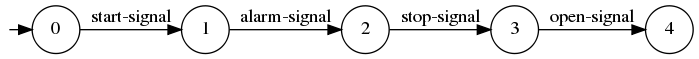
\includegraphics{src/2-framework/images/local-trace}}
\caption{LTS capturing the traces of the MSC in Fig.~\ref{image:train-scenario-all-agents} from the local point of view of the \artifact{Controller}.\label{image:local-traces-lts}}
\end{figure}

When looking at traces from the perspective of the whole MSC, two possibilities might be envisaged.

\noindent \textbf{Total event ordering} -- one might consider that a MSC defines a simple \emph{maximal} trace where all events appear according to the graphical top-down ordering. In our example, such trace would be

\begin{center}\artifact{<start-signal, start, alarm-pressed, \ldots, open>}\end{center} 

A MSC would then define a total order among all events. This leads to a simple and straightforward, yet limited, trace semantics for MSCs.

\noindent \textbf{Partial event ordering} -- when considering concurrent systems, a partial ordering among events seems more adequate~\cite{ITU:1996, Uchitel:2003}. Consider for example the events \artifact{start-signal} and \artifact{alarm-pressed} at the beginning of the MSC shown in Fig.~\ref{image:train-scenario-all-agents}. These two events capture unrelated message passing between different agents; they can therefore hardly be considered ordered over time -- e.g. the passenger might push the alarm button when the \artifact{start-signal} is already sent but before \artifact{start} has been propagated; or maybe even before \artifact{start-signal}; and so on. 

To account for such situations, one has to consider that the traces defined by a MSC are \emph{linearizations} of the partial order among MSC events. In other words, linearizations capture all possible sequences of events that respect the total ordering defined by the timelines. We do not formalize the structure of Message Sequence Charts and their linearizations here, and refer the reader to~\cite{Uchitel:2003} for such a mathematical characterization. 

The set of traces obtained from the local and global perspectives discussed are related ass follows:

\vspace{-0.4cm}
\begin{equation}
\label{equation:msc-composition}
\mathcal{L}_{total}(M) \subseteq \mathcal{L}_{partial}(M) \\
\mathcal{L}_{partial}(M) = \mathcal{L}(M_{\downarrow Ag_1} \parallel \ldots \parallel M_{\downarrow Ag_n})
\end{equation}

The left part simply states that traces under a partial ordering certainly include those under a total ordering, which is expected. Indeed, the model with partial ordering is more general than the one with total ordering. Among others, it means that everything that is true for the former is certainly true for the latter as well. From now on, and unless stated otherwise, we therefore assume the general model with partial ordering. In particular, we do not make the $partial$ and $total$ subscripts explicit when stating other language relations in the following sections. A consistent use of one of them renders all formula valid.

The right part provides a simple way of computing all linearizations of a MSC as an (acyclic) transition system, through LTS composition. Such a LTS is illustrated in Fig.~\ref{image:msc-linearizations} for the MSC of Fig.\ref{image:train-scenario-all-agents}. As shown, the latter accepts six different linearizations, due to the possible interleaving of its first four events. By construction, such a LTS has only one initial state (the leftmost one) and only one terminating state (the rightmost one). This allows us to loosely refer to \emph{the} terminating state of an MSC (more precisely, of the LTS capturing its traces) with a precise underlying meaning.

\aside{The reader wondering whether certain linearizations are not \emph{implied} scenarios~\cite{Uchitel:2004} or whether our initial scenario should not be regarded flawed is referred to Section~\ref{section:background-discussion} where those issues are further examined.}

\begin{figure}\centering
\scalebox{0.31}{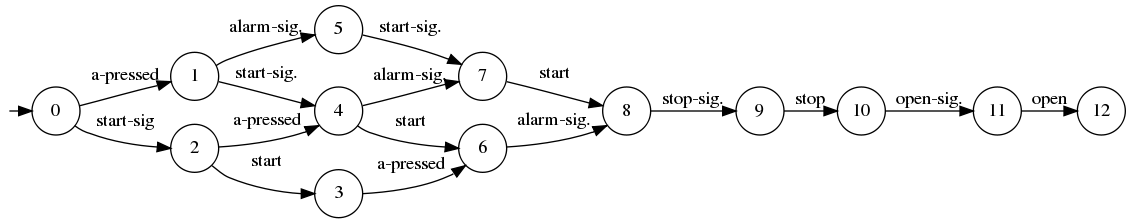
\includegraphics{src/2-framework/images/linearizations}}
\caption{LTS capturing all event linearizations of the MSC of Fig.~\ref{image:train-scenario-all-agents}. Here, \artifact{alarm-pressed} is abbreviated as \artifact{a-pressed} and \artifact{sig.} stands for \artifact{signal}. \label{image:msc-linearizations}}
\end{figure}

\subsubsection*{Multi-view model consistency}

The trace semantics of a single MSC can now be explicitly related to the notions of agent and system behaviors, also captured with LTSs in Section~\ref{section:background-state-machines}. This amounts to define consistency rules between them, and explains the similitude between definitions \ref{equation:system-composition} and \ref{equation:msc-composition}.

Consider a system composed of $n$ agents whose behavior is modeled as $\system$. Let $M$ denote a MSC illustrating interactions between them. We say that $M$ is \emph{consistent} with $S$ -- or, more accurately, that $M$ and $S$ \emph{are} consistent -- if the following conditions hold:

\begin{itemize}
\item $M$ and $S$ are \emph{architecturally} consistent,
\item $\mathcal{L}(M_{\downarrow Ag_i}) \subseteq \mathcal{L}(Ag_i)$ for each agent $Ag_i$, and
\item $\mathcal{L}(M) = \mathcal{L}(M_{\downarrow Ag_1} \parallel \ldots \parallel M_{\downarrow Ag_n}) \subseteq \mathcal{L}(Ag_1 \parallel \ldots \parallel Ag_n) = \mathcal{L}(S)$
\end{itemize}

The first condition is not formalized but simply requires the MSC and the system to agree on the set of agents (a MSC may actually illustrate interactions among a proper subset of system agents) and their respective interfaces (labels along a timeline are a subset of the alphabet of the corresponding agent). The second condition states that the traces defined by a timeline in the MSC must be traces accepted in the LTS modeling the behavior of the corresponding agent. The third condition states that all linearizations of the MSC must be accepted traces of the LTS modeling the behavior of the composed system. Note that, under architectural consistency, the second condition implies the third one~\cite{Uchitel:2003}. Last, but not least, stated conditions restrict consistent MSCs to those starting in the system initial state.

\subsection{Negative scenarios\label{subsection:background-negative-scenarios}}

While positive MSCs model examples of behavior that the system is expected to exhibit, it is often convenient to be able to model the counterpart, that is examples of behavior that the system is expected (even required) \emph{not} to exhibit. Such proscribed behaviors are illustrated with negative MSCs~\cite{Uchitel:2004}. A negative MSC is simply a scenario whose last event is proscribed, as depicted by a crossed arrow below a dashed line. An example is given in Fig.~\ref{image:train-negative-scenario}, where the \artifact{Controller} may not open doors immediately after having started the train.

\begin{figure}\centering
\scalebox{0.75}{
  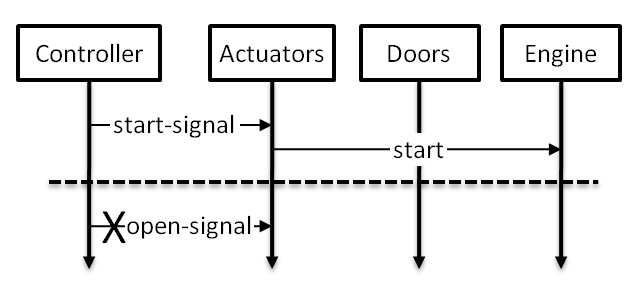
\includegraphics[trim=2mm 2mm 2mm 2mm, clip]{src/2-framework/images/train-negative-scenario}
}
\caption{A negative scenario illustrating that the controller may not open doors after having started.\label{image:train-negative-scenario}}
\end{figure}

More precisely, a negative MSC is a pair $(P,e)$ where $P$ is a positive MSC and $e$ is a single event (given our simplifying assumption, the latter event can simply be denoted by its label $l = label(e)$). The positive scenario $P$ is called the $precondition$ and $e$ the \emph{proscribed event}. The intuitive semantics is that, once the precondition has occurred from the system initial state, $e$ may not be the (very) \emph{next} event in the system. We make this semantics fully precise now. First, if the precondition of a negative MSC $N = (P,e)$ is a positive MSC, it certainly defines sets of positive traces:

\vspace{-0.2cm}
\begin{equation*}
\mathcal{L}^{+}(N) = \mathcal{L}(P)
\end{equation*}

\noindent In addition, it defines the following set of negative traces:

\vspace{-0.2cm}
\begin{equation*}
\mathcal{L}^{-}(N) = \{~w.l \mid w \in mt(\mathcal{L}(P)) \wedge l = label(e)~\}
\end{equation*}

That is, negative traces are maximal traces of the precondition concatenated with the label of the proscribed event. Note that such a definition implies that the precondition must occur completely for the proscribed event to be taken into account. In other words, partial orderings between the proscribed event and those in the precondition are never considered. This is the intended meaning of the dashed line separating them~\cite{Uchitel:2004}. 

Last, observe that the set of negative traces cannot be captured with the sole mean of a LTS. This is because $\mathcal{L}^{-}(N)$ is not prefix-closed (see Section~\ref{section:background-lts-and-regular-languages}). Negative scenarios are sometimes captured by a LTS extended with an error state~\cite{Uchitel:2004}. Another way consists in using a standard automaton, which makes a distinction between accepting and non-accepting states. 

\subsubsection*{Multi-view model consistency}

Similarly to positive MSCs, we state conditions for a negative MSC $N = (P,e)$ and a system $\system$ to be consistent, as follows:

\begin{itemize}
\item $N$ and $S$ are \emph{architecturally} consistent,
\item $P$ and $S$ are consistent, and
\item $\mathcal{L}^{-}(N) \not\subseteq \mathcal{L}(Ag_1 \parallel \ldots \parallel Ag_n) = \mathcal{L}(S)$
\end{itemize}

The first condition is similar to what has been said previously for positive MSCs. The second enforces the precondition to be a consistent (positive) MSC, implicitly requiring positive traces to be accepted. The last one states that the system may not exhibit any negative trace captured by the negative MSC.

\subsection{Scenario collections\label{subsection:background-scenario-collections}}

Systems are generally illustrated with multiple positive and negative scenarios. The most straightforward way of doing so is through a scenario collection $Sc = (S^+,S^-)$ where $S^+$ and $S^-$ are finite (but possibly empty) sets of positive MSCs and negative MSCs, respectively. It is straightforward, yet useful, to extend the notions of language and consistency of scenarios to collections of them. 

The positive and negative languages defined by a scenario collection $Sc = (S^+,S^-)$ are simply defined via the union on languages, but taking into account the fact that negative scenarios define positive traces in addition to negative ones:

\vspace{-0.5cm}
\begin{align*}
\mathcal{L}^+(Sc) &= \bigcup_{P \in S^+} \mathcal{L}(P)~~\cup~~\bigcup_{N \in S^{-}} \mathcal{L}^{+}(N) \\
\mathcal{L}^-(Sc) &= \bigcup_{N \in S^-} \mathcal{L}^{-}(N)
\end{align*}

Also, a scenario collection and a system are said to be consistent if and only if each positive and each negative MSC of the collection is itself consistent with the system. We extend this to the consistence of the collection of scenarios itself as follows: two sets of positive and negative scenarios, $S^+$ and $S^-$, are consistent with each other if there exists a system which is consistent with them taken as a collection $Sc = (S^+,S^-)$. A necessary condition for a scenario collection to be consistent (but not sufficient, because architectural consistency is not taken into account here) is the disjointness of positive and negative traces:

\begin{center}
$Sc = (S^+,S^-)$ is consistent only if $\mathcal{L}^+(Sc) \cap \mathcal{L}^-(Sc) = \emptyset$
\end{center}

Note that, by definition, a collection cannot be consistent with a system unless all scenarios start in its initial state. Also, since scenarios and scenario collections are both finite, a collection is hardly complete in practice because most systems accept an infinite number of traces, through loops. Last, the fact that all scenarios must start in the same initial state may imply a lot of redundancy in descriptions of large systems. Among others, this can render consistency difficult to guarantee unless costly refactoring steps are conducted on scenarios. High-level Message Sequence Charts (hMSCs), introduced in the next section, provide a mean to tackle these problems.

\subsection{Flowcharting scenarios in high-level message sequence charts\label{section:background-hmsc}}

A High Level Message Sequence Chart is a directed graph where each node refers to a MSC (named \emph{basic} MSC, bMSC for short) or a finer grained hMSC~\cite{ITU:1996}. We ignore this later possibility until further notice. Outgoing edges of a node capture its possible continuations, allowing the user to introduce sequences, alternatives and loops, to reuse small MSC fragments, and so on. An hMSC also has an initial starting point that indicates the initial system state. An example of hMSC is given in Fig.~\ref{image:train-hmsc}. 

\vspace{0.4cm}
\begin{figure}[H]\centering
\scalebox{0.66}{
  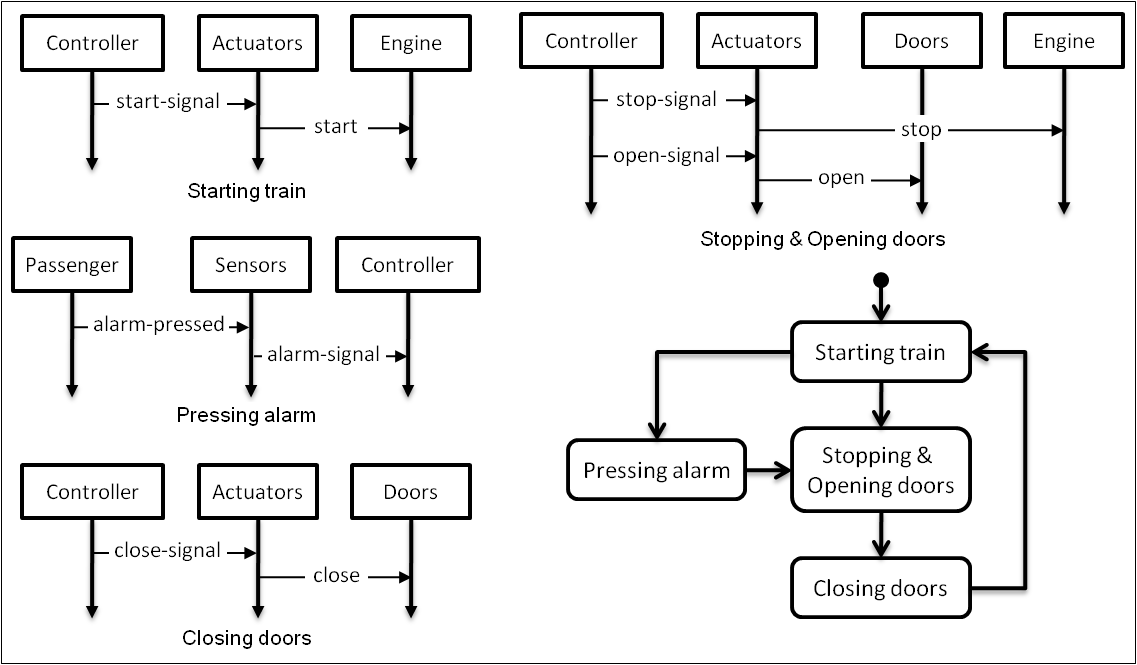
\includegraphics[trim=2mm 2mm 2mm 2mm, clip]{src/2-framework/images/train-hmsc}
}
\caption{A high-level Message Sequence Chart for the train system.\label{image:train-hmsc}}
\end{figure}

A trace semantics can of course be given to hMSCs, which amounts to answering the question \emph{what traces are captured by a hMSC?} This apparently simple question has, however, a more complex answer. The reasons are actually manifold; we summarize here, and slightly extend, the characterization given in~\cite{Uchitel:2004}.

First of all, some hMSCs do not define regular languages~\cite{Henriksen:2000}, and therefore have sets of traces that cannot be modeled with LTS. Therefore, we must restrict our framework to regular hMSCs. Under total ordering of events inside bMSCs, hMSCs are regular. Under partial ordering, a sufficient condition for being regular is that the hMSC does not contain a cycle in which two disjoint sets of agents interact independently of each other. We assume such \emph{bounded} hMSCs in the sequel. 

Also, in addition to the partial or total ordering of events in bMSCs, two interpretations co-exist about how a system evolves from a bMSC to another inside a hMSC. The first one, called \emph{strong sequential composition}, is to assume that all agents wait until all events of a bMSC have occurred before moving on to the next one. This implies that there is an implicit synchronization scheme used by agents to know when a scenario has been completed. The other one, \emph{weak sequential composition}, does not make such an assumption and allows an agent to move from a bMSC to another one without having to synchronize with the other agents. Given the independence between assumptions of partial/total event ordering and weak/strong sequential composition, four combinations actually exist. To keep things simple enough, and because they lead to strange concurrency models\footnote{in particular, one can check that such models are very sensitive to bMSC concatenation and decomposition}, we do not consider partial (resp. total) ordering with strong (resp. weak) sequential composition. In the sequel, therefore, strong (resp. weak) sequential composition implies total ordering (resp. partial) of MSC events.

Under these assumptions, the trace analysis for hMSCs is very similar to what has been done for MSCs, and therefore leads to language relations similar to the ones given for the latter in Section~\ref{subsection:background-positive-scenarios} (see equation~\ref{equation:msc-composition}):

\begin{equation}
\mathcal{L}_{strong}(H) \subseteq \mathcal{L}_{weak}(H) \subseteq \mathcal{L}(H_{\downarrow Ag_1} \parallel \ldots \parallel H_{\downarrow Ag_n})
\label{equation:hsmc-traces-by-agent-composition}
\end{equation}

The set of traces $\mathcal{L}_{strong}(H)$ and $\mathcal{L}_{weak}(H)$ are easily explained by considering scenarios ``built'' by the hMSC. Consider a finite path in the hMSC. Concatenating the bMSCs along this path ``builds'' a single MSC. For example, concatenating \artifact{Starting train}, \artifact{Pressing alarm} and \artifact{Stopping \& Opening the doors} in the hMSC of Fig.~\ref{image:train-hmsc} leads to the MSC of Fig.~\ref{image:train-scenario-all-agents}. From results in Section~\ref{subsection:background-positive-scenarios}, such a MSC $M$ defines the set of traces $\mathcal{L}_{total}(M)$ and $\mathcal{L}_{partial}(M)$. To define traces defines by a hMSC $H$, we have to consider all such possible MSCs: 

\vspace{-0.5cm}
\begin{align*}
\mathcal{L}_{strong}(H) &= \bigcup_{M \in H} \mathcal{L}_{total}(M) \\
\mathcal{L}_{weak}(H) &= \bigcup_{M \in H} \mathcal{L}_{partial}(M)
\end{align*}

%\vspace{-0.8cm}
\noindent where $M \in H$ means ``the MSC $M$ can be built by $H$'', with the obvious meaning in terms of possible paths in $H$. The language $\mathcal{L}_{weak}$ corresponds to the notion of \emph{trace model} in~\cite{Uchitel:2004}.

Now, one can actually consider another way to compute the set of traces defined by a hMSC. In this alternative way, the local perspective of the agent timelines is taken into account, in a way similar to what has been done for MSCs. This leads to the rightmost part of the relations between hMSC languages in~\ref{equation:hsmc-traces-by-agent-composition}, that computes hMSC traces as the composition of local agent traces $H_{\downarrow Ag_i}$. The composition of such a LTS for each agent correspond to the notion of \emph{minimal architecture model} in~\cite{Uchitel:2004} and will sometimes be denoted by $\mathcal{L}_{arch}(H)$.

An algorithm can be found in~\cite{Uchitel:2004} for synthesizing the LTS modeling $\mathcal{L}_{arch}(H)$. For a given agent $Ag_{i}$, the LTS $H_{\downarrow Ag_i}$ is synthesized by connecting the LTSs $M_{\downarrow Ag_i}$ corresponding to each bMSC $M$ with $\tau$ transitions, according to their possible continuations given by hMSC edges. This construction is illustrated in Fig.~\ref{image:train-controller-synthesis} for the hMSC of Fig.~\ref{image:train-hmsc} and the \artifact{Controller} agent. The resulting LTS can be further simplified by removing $\tau$ transitions and minimizing the LTS.  Note that, thanks to the simplicity of the model with strong sequential composition, $\mathcal{L}_{strong}(H)$ can be computed in a very similar way. In contrast, $\mathcal{L}_{weak}(H)$ is much harder to model as a LTS; a synthesis algorithm can however be found in~\cite{Uchitel:2004}.

\vspace{0.4cm}
\begin{figure}[H]\centering
\scalebox{0.85}{
  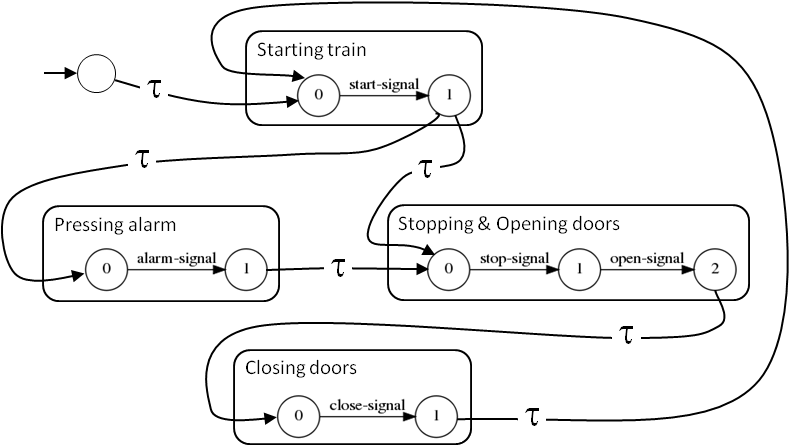
\includegraphics[trim=0mm 0mm 0mm 0mm, clip]{src/2-framework/images/train-controller-synthesis}
}
\caption{Synthesis of the \emph{Controller} LTS from the hMSC of Fig.~\ref{image:train-hmsc}.\label{image:train-controller-synthesis}}
\end{figure}

One can note an important difference between the relations between MSC languages in~\ref{equation:msc-composition} and those between hMSC languages in~\ref{equation:hsmc-traces-by-agent-composition}. Indeed, the former denotes an equality between $\mathcal{L}_{partial}(M)$ and $\mathcal{L}(M_{\downarrow Ag_1}\parallel\ldots\parallel M_{\downarrow Ag_n})$ while the latter defines a set inclusion between $\mathcal{L}_{weak}(H)$ and $\mathcal{L}(H_{\downarrow Ag_1}\parallel\ldots\parallel H_{\downarrow Ag_n})$. In fact, traces in $\mathcal{L}_{arch}(H) \setminus \mathcal{L}_{weak}(H)$ capture the set of \emph{implied} scenarios of a hMSC specification~\cite{Alur:2000, Uchitel:2004}. Implied scenarios occur when a system is designed globally (the hMSC) while implemented component-wise (the composition of agent LTSs). In other words, implied scenarios capture traces that follow different paths in the hMSC when projected on individual agent timelines. We come back to them in Section~\ref{section:background-discussion}.

\subsubsection*{Finer-grained hMSC}

As stated previously, a hMSC node can refer to a finer-grained hMSC instead of a bMSC. Taken them into account in the trace semantics given previously requires deciding how a sub-hMSC has to be ``connected'' with its father. To keep a consistent framework in terms of synchronization hypotheses, we require such a sub-hMSC to have, in addition to its initial state, a terminating state to which at least one node is connected. For simplicity, we also forbid nodes with no outgoing transition. Under such assumptions, it is relatively easy to ``unfold'' a hMSC as another one with all nodes refined as basic MSCs. The trace semantics remains unchanged and is defined in terms of the latter ``flat'' hMSC. 

In practice, this flat hMSC must not be explicitly constructed when synthesizing the LTS for $\mathcal{L}_{arch}$. Indeed, the LTSs $H_{\downarrow Ag_i}$ of finer-grained hMSCs respecting our constraints present only one initial state and only one terminating state, allowing them to be connected with $\tau$ transitions in the same way than LTSs $M_{\downarrow Ag_i}$. Similar argument applies for $\mathcal{L}_{strong}$, but not for $\mathcal{L}_{weak}$.

\subsubsection*{Multi-view model consistency}
 
Based on the trace semantics defined in the previous section, we can now define additional consistency rules in our framework. We say that a hMSC $H$ and a system $\system$ are consistent if the following condition holds:

\begin{itemize}
\item $H$ and $S$ are \emph{architecturally} consistent,
\item $\mathcal{L}(H_{\downarrow Ag_i}) \subseteq \mathcal{L}(Ag_i)$ for each agent $Ag_i$, and
\item $\mathcal{L}_{arch}(H) = \mathcal{L}(H_{\downarrow Ag_1} \parallel \ldots \parallel H_{\downarrow Ag_n}) \subseteq \mathcal{L}(Ag_1 \parallel \ldots \parallel Ag_n) = \mathcal{L}(S)$
\end{itemize}

These conditions are the counterpart of those given previously for MSCs and have a similar interpretation, \emph{mutatis mutandis}. In addition, however, it is convenient to distinguish between a hMSC that describes all behaviors of a system and one that only illustrates a subset of them. This leads to the notion of hMSC completeness. A hMSC $H$ is \emph{complete} for a system $\system$ if it is consistent with it and defines the same language, that is, if $\mathcal{L}_{arch}(H) = \mathcal{L}(S).$

\subsection{Explicit state annotations\label{subsection:background-scenario-annotations}}

A last construction allowed in MSCs is worth discussing that helps managing multiple scenarios. Indeed, many authors allow MSCs to be annotated with state-based information (see, e.g.,~\cite{Kruger:2000, Whittle:2000}). 

TODO: complete this description, discussing the difference between identification and state assertions (aka fluent-based decorations). The former info uniquely identifies an agent state, so that they can be merged with mandatory merge constraints presented in section~\ref{section:inductive-from-hMSC}, while the later does not, but helps pruning search space as usual with fluents.
